\documentclass{article}
\usepackage[utf8]{inputenc}
\usepackage[includeheadfoot, margin=1em,headheight=2em]{geometry}
\usepackage{titling}
\geometry{a4paper, left=2cm, right=2cm, top=2cm, bottom=2cm}
\usepackage{graphicx}
\usepackage{float}
\providecommand{\versionnumber}{1.0.0}
\usepackage{enumitem}
\usepackage{array}
\usepackage[italian]{babel}
\newcolumntype{P}[1]{>{\centering\arraybackslash}p{#1}}
\renewcommand{\arraystretch}{1.5} % Default value: 1
\setlength{\droptitle}{-6em}

%font
\usepackage[defaultfam,tabular,lining]{montserrat}
\usepackage[T1]{fontenc}
\renewcommand*\oldstylenums[1]{{\fontfamily{Montserrat-TOsF}\selectfont #1}}

%custom bold 
\usepackage[outline]{contour}
\usepackage{xcolor}
\newcommand{\custombold}{\contour{black}}

%table colors
\usepackage{color, colortbl}
\definecolor{Blue}{rgb}{0.51,0.68,0.79}
\definecolor{LightBlue}{rgb}{0.82,0.87,0.90}
\definecolor{LighterBlue}{rgb}{0.93,0.95,0.96}

%Header
\usepackage{fancyhdr, xcolor}
\pagestyle{fancy}
\let\oldheadrule\headrule% Copy \headrule into \oldheadrule
\renewcommand{\headrule}{\color{Blue}\oldheadrule}% Add colour to \headrule
\renewcommand{\headrulewidth}{0.2em}
\fancyhead[L]{Analisi Celonis}
\fancyhead[C]{Samuele Vignotto}
\fancyhead[R]{
\includegraphics[height=1cm]{Logo/Y_LOGO-SOLO.png}}
\setcounter{secnumdepth}{0}

\title{\Huge{\textbf{Analisi della piattaforma di process mining Celonis}}\vspace{-1em}}
\author{Samuele Vignotto}
\date{}
\begin{document}
\maketitle
\begin{figure}[h]
  \centering
  
\includegraphics[width=6cm, height=6cm]{Logo/Y_LOGO-SOLO.png}
  \label{fig:immagine}
\end{figure}

\newpage
\tableofcontents
\newpage

\section{Introduzione}

Il process mining è una disciplina emergente che combina tecniche di data mining e di analisi dei processi aziendali per fornire una visione approfondita dei processi operativi di un'organizzazione. Una delle piattaforme leader in questo campo è Celonis, una soluzione di process mining avanzata che permette alle aziende di ottimizzare e migliorare continuamente i propri processi aziendali.

\subsection{Estrazione Automatica dei Dati}

Celonis si distingue per la sua capacità di estrarre automaticamente dati da vari sistemi informatici aziendali, tra cui ERP (Enterprise Resource Planning), CRM (Customer Relationship Management) e altri sistemi transazionali. Utilizzando queste informazioni, Celonis crea una rappresentazione visiva e dettagliata dei processi aziendali reali, consentendo agli utenti di identificare inefficienze, colli di bottiglia e deviazioni dai processi standard.

\subsection{Analisi in Tempo Reale}

Una delle funzionalità chiave di Celonis è la sua capacità di fornire un'analisi in tempo reale. Questa caratteristica permette alle organizzazioni di monitorare i propri processi in modo continuo, rilevando e risolvendo problemi immediatamente. Inoltre, Celonis offre potenti strumenti di visualizzazione che permettono agli utenti di esplorare i dati da diverse prospettive, identificando facilmente le aree critiche che necessitano di miglioramenti.

\subsection{Benchmarking}

Un altro aspetto fondamentale di Celonis è la sua funzione di benchmarking, che consente alle aziende di confrontare le proprie prestazioni con quelle di altre organizzazioni o con standard di settore. Questo confronto aiuta a identificare le migliori pratiche e a impostare obiettivi di miglioramento realistici.

\subsection{Integrazione con Machine Learning e Intelligenza Artificiale}

Celonis supporta anche l'integrazione con tecniche di machine learning e intelligenza artificiale, permettendo di prevedere l'andamento dei processi e di suggerire azioni correttive proattive. Questo approccio predittivo è particolarmente utile per anticipare problemi potenziali e mitigare rischi operativi.

\subsection{Automazione dei Processi}

Inoltre, Celonis offre funzionalità di automazione dei processi, che permettono di implementare rapidamente miglioramenti identificati attraverso il process mining. Questo porta a una riduzione dei tempi di ciclo, a una maggiore conformità e a un miglioramento generale dell'efficienza operativa.


\section{Integrazione dei dati}
I dati che la piattaforma Celonis utilizza sono catturati dagli strumenti e dai sistemi aziendali (definiti come sistemi sorgente). Questi sistemi sorgente possono essere integrati con la piattaforma Celonis, permettendo di estrarre i dati rilevanti, trasformarli secondo le esigenze e di caricarli in un modello di dati per essere utilizzati in tutta la piattaforma.

\begin{figure}[H]
    \centering
    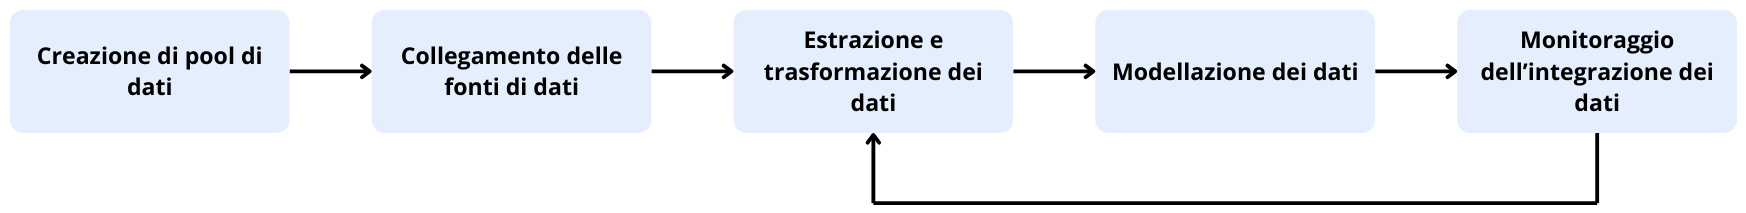
\includegraphics[width=\textwidth]{imgCelonis/IntegrazioneDati.png}
    \caption{Flusso dell'integrazione dati in Celonis}
    \label{fig:flusso-integrazione-dati-celonis}
\end{figure}

\subsection{Creazione e manutenzione di pool di dati}
Un pool di dati è l'elemento strutturale principale del flusso di lavoro di integrazione dei dati. Serve da contenitore per le fonti di dati e facilita il monitoraggio dei dati.

\subsubsection{Tipi di dati necessari}
La piattaforma richiede vari tipi di dati, tra cui file di log degli eventi, fogli di calcolo (Google Sheets, CSV, XLSX), flussi di eventi estensibili (XES) e dati da applicazioni enterprise come SAP, Oracle EBS, Salesforce, e ServiceNow. Inoltre, supporta fonti di dati cloud e database tradizionali come Microsoft SQL, Oracle e Snowflake. L'integrazione con queste fonti è facilitata da connettori specifici e dall'utilizzo di API.\\
Celonis offre connettori specifici per Oracle Database, che consentono l'estrazione dei dati direttamente dalle tabelle e dalle viste, garantendo la coerenza e l'aggiornamento continuo delle informazioni. Questo processo include la gestione di schemi complessi e l'ottimizzazione delle query per ridurre l'impatto sulle prestazioni del database di origine.\\
Per quanto riguarda i sistemi ERP, Celonis supporta l'integrazione con soluzioni come SAP e Oracle E-Business Suite. L'estrazione dei dati da questi sistemi prevede l'utilizzo di API e connettori dedicati, che facilitano la raccolta di dati transazionali e master. Questo consente di ottenere una visione completa dei processi aziendali, dalla gestione degli ordini alla supply chain, migliorando così l'analisi e l'ottimizzazione dei processi.

\subsubsection{Vantaggi della piattaforma}
Uno dei principali vantaggi di Celonis è la sua capacità di connettersi a una vasta gamma di fonti di dati, sia on-premise che cloud, offrendo molta flessibilità. La piattaforma permette l'estrazione in tempo reale dei dati, garantendo che le analisi siano sempre basate su informazioni aggiornate. Inoltre, Celonis supporta la trasformazione dei dati con strumenti integrati, semplificando il processo di preparazione dei dati per l'analisi.

\subsubsection{Svantaggi della Piattaforma}
L'integrazione dei dati in Celonis può presentare alcune sfide. L'aggiornamento e la manutenzione delle connessioni ai vari sistemi possono risultare complessi, soprattutto in ambienti IT eterogenei. Infine, l'uso intensivo di risorse durante i processi di estrazione e trasformazione può influire sulle prestazioni dei sistemi coinvolti.

\section{Implementazioni pratiche di inserimento dei dati: simulazioni}
\subsection{Prima simulazione}
\subsubsection{Struttura del file CSV}
Il file CSV con i dati simulati contiene informazioni riguardanti le attività di una ditta che riceve prodotti da un'azienda, li vende online e li spedisce ai clienti. La struttura del file è la seguente:
\begin{itemize}
    \item \custombold{activity\_id}: identificativo univoco per ogni attività;
    \item \custombold{activity}: nome dell'attività svolta;
    \item \custombold{timestamp}: data e ora in cui l'attività è stata svolta;
    \item \custombold{product\_id}: identificativo del prodotto coinvolto nell'attività.
\end{itemize}
Esempio di contenuto del file CSV:
\begin{table}[htbp]
    \centering
    \begin{tabular}{|c|c|c|c|}
        \hline
        \textbf{activity\_id} & \textbf{activity} & \textbf{timestamp} & \textbf{product\_id} \\
        \hline
        1 & Receive Goods & 2023-08-02 18:20:10.465195 & 1 \\
        \hline
        2 & Quality Check & 2023-12-03 13:30:22.465195 & 1 \\
        \hline
        3 & Store in Warehouse & 2024-03-09 18:03:55.465195 & 1 \\
        \hline
        4 & Pick for Order & 2024-03-15 02:03:15.465195 & 1 \\
        \hline
        5 & Order Cancellation & 2024-05-29 08:01:26.465195 & 1 \\
        \hline
    \end{tabular}
    \caption{Activity Log}
    \label{tab:activity_log}
\end{table}
\subsubsection{Regole di simulazione dei dati}
I dati simulati sono stati generati seguendo determinate regole per garantire la coerenza temporale e la rappresentazione realistica dei processi aziendali. Le regole principali sono:
\begin{itemize}
    \item \custombold{Coerenza dei Timestamps}: I timestamp delle attività devono essere coerenti. Ad esempio, il timestamp della spedizione al cliente non può essere precedente al timestamp dell'ordine.
    \item \custombold{Cicli di attività possibili}:
    \begin{itemize}
        \item \custombold{Ciclo 1}: Receive Goods -> Quality Check -> Store in Warehouse
        \item \custombold{Ciclo 1}: Receive Goods -> Quality Check -> Store in Warehouse -> Pick for Order -> Order Cancellation
        \item \custombold{Ciclo 1}: Receive Goods -> Quality Check -> Store in Warehouse -> Pick for Order -> Receive Payment -> Pack for Shipment -> Ship to Customer -> Customer Receive Goods
        \item \custombold{Ciclo 1}: Receive Goods -> Quality Check -> Store in Warehouse -> Pick for Order -> Receive Payment -> Pack for Shipment -> Ship to Customer -> Customer Receive Goods -> Customer Feedback
        \item \custombold{Ciclo 1}: Receive Goods -> Quality Check -> Store in Warehouse -> Pick for Order -> Receive Payment -> Pack for Shipment -> Ship to Customer -> Customer Receive Goods -> Customer Feedback -> Return Processing
    \end{itemize}
\end{itemize}
\subsubsection{Analisi delle attività}
Le attività principali e la loro frequenza nei dati simulati sono le seguenti:
\begin{itemize}
    \item \custombold{Receive Goods}: 100\% dei casi;
    \item \custombold{Quality Check}: 100\% dei casi;
    \item \custombold{Store in Warehouse}: 100\% dei casi;
    \item \custombold{Pick for Order}: 84\% dei casi;
    \item \custombold{Customer Receive Goods}: 68\% dei casi;
    \item \custombold{Pack for Shipment}: 68\% dei casi;
    \item \custombold{Receive Payment}: 68\% dei casi;
    \item \custombold{Ship to Customer}: 68\% dei casi;
    \item \custombold{Customer Feedback}: 41\% dei casi;
    \item \custombold{Return Processing}: 31\% dei casi;
\end{itemize}
\subsubsection{Analisi del processo}
Il file CSV è stato utilizzato per testare diverse funzionalità della piattaforma Celonis, fornendo una visione chiara del flusso di lavoro aziendale e delle sue inefficienze.\\
Inizialmente, abbiamo esplorato la funzione "What does your process look like?", analizzando un totale di 100 casi distribuiti tra luglio 2023 e luglio 2024. Questa analisi ci ha permesso di osservare la variazione mensile dei casi, evidenziando come questi siano distribuiti lungo l'anno. Inoltre, sono stati identificati 11 processi distinti, con frequenze specifiche per ciascuna attività all'interno del processo.\\
\begin{figure}[H]
    \centering
    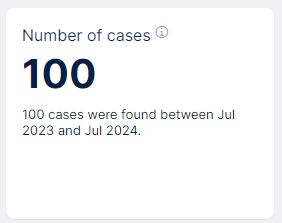
\includegraphics[width=0.33\textwidth]{imgCelonis/PrimaSimulazione/NumeroCasi.png}
    \caption{Numero di casi identificati da Celonis}
    \label{fig:Casi-Identificati_Celonis}
\end{figure}
\begin{figure}[H]
    \centering
    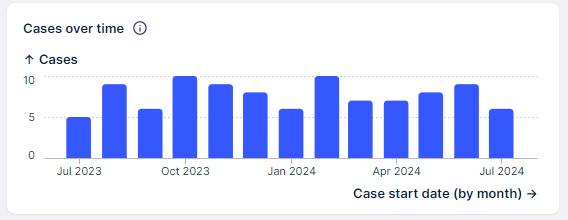
\includegraphics[width=0.33\textwidth]{imgCelonis/PrimaSimulazione/DistribuzioneCasiMesi.png}
    \caption{Distribuzione dei casi identificata da Celonis}
    \label{fig:Distribuzione-Casi_Celonis}
\end{figure}
\begin{figure}[H]
    \centering
    \includegraphics[width=0.33\textwidth]{imgCelonis/PrimaSimulazione/NumeroAttività.png}
    \caption{Numero di attività identificate da Celonis}
    \label{fig:Attività-Identificate-Celonis}
\end{figure}
La visualizzazione grafica generata da Celonis ha mostrato chiaramente le sequenze delle attività, permettendoci di comprendere meglio il flusso dei processi aziendali. I filtri disponibili ci hanno consentito di personalizzare la visualizzazione, focalizzandoci su dettagli specifici dei casi e delle attività.\\
\begin{figure}[H]
    \centering
    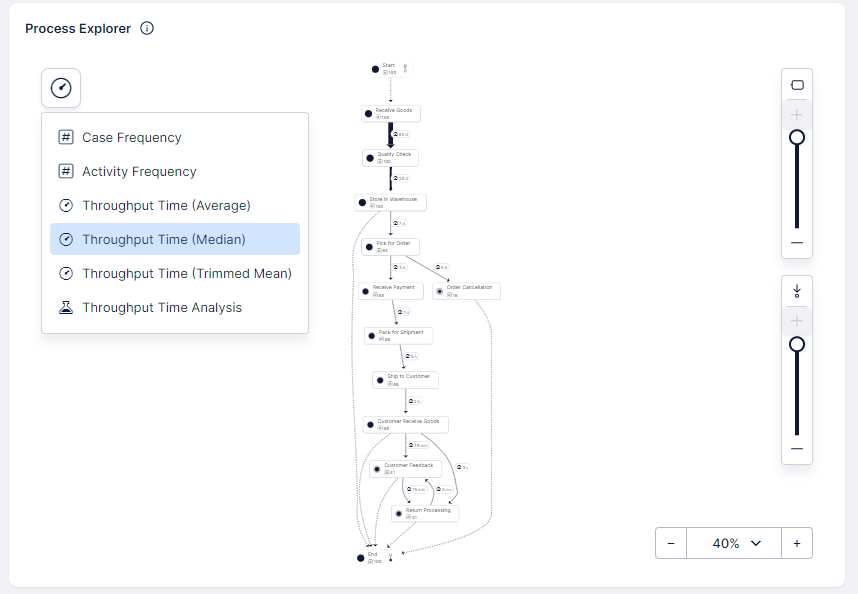
\includegraphics[width=\textwidth]{imgCelonis/PrimaSimulazione/GrafoSimulazione.png}
    \caption{Grafo del processo creato da Celonis}
    \label{fig:Grafo-processo_Celonis}
\end{figure}
Passando alla sezione "How long does your process take?", abbiamo esaminato i tempi di esecuzione delle attività dall'inizio alla fine del processo, fornendo una chiara distribuzione temporale dei casi. Questa analisi ha permesso di identificare le connessioni con ampie distribuzioni di Throughput Times, rivelando inefficienze significative.\\
\begin{figure}[H]
    \centering
    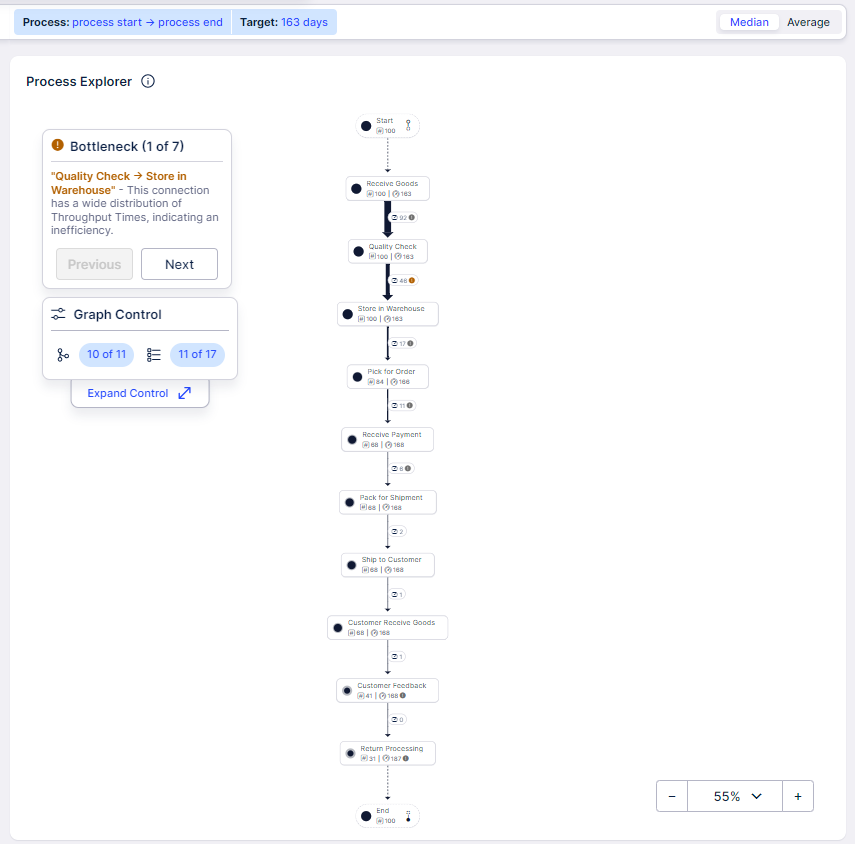
\includegraphics[width=\textwidth]{imgCelonis/PrimaSimulazione/GrafoColliDiBottiglia.png}
    \caption{Grafo del processo con evidenziati i colli di bottiglia}
    \label{fig:Grafo-colli-di-bottiglia}
\end{figure}
Celonis ha identificato vari colli di bottiglia nei dati simulati. Tra questi, la connessione tra Quality Check e Store in Warehouse ha mostrato una distribuzione ampia dei tempi di esecuzione, indicando un'inefficienza. Analoghe osservazioni sono state fatte per le connessioni tra Receive Goods e Quality Check, Store in Warehouse e Pick for Order, Receive Payment e Pack for Shipment, Pick for Order e Receive Payment. Inoltre, le attività di Customer Feedback e Return Processing hanno mostrato tempi di esecuzione elevati, contribuendo ulteriormente alle inefficienze del processo.\\
\begin{figure}[H]
    \centering
    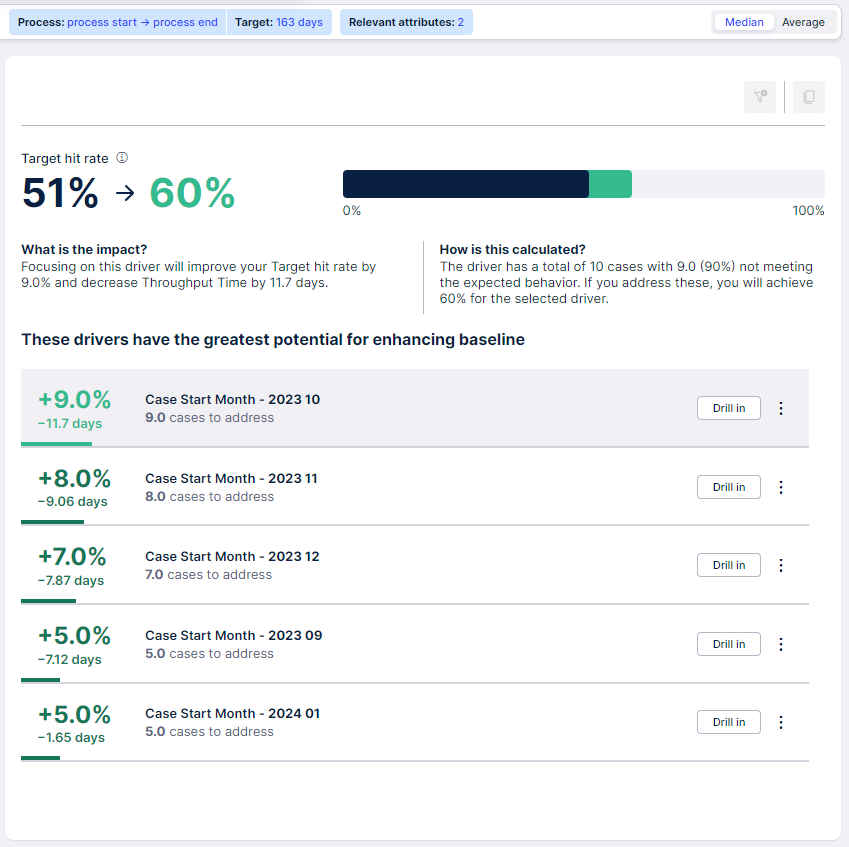
\includegraphics[width=\textwidth]{imgCelonis/PrimaSimulazione/MiglioramentiSuggeriti.png}
    \caption{Miglioramenti suggeriti da Celonis}
    \label{fig:Miglioramenti-suggeriti}
\end{figure}
Questa analisi approfondita ha evidenziato come Celonis possa identificare i punti deboli nei processi aziendali e suggerire miglioramenti concreti, contribuendo a ottimizzare l'efficienza operativa complessiva.
\subsubsection{Conclusioni}
Il file con i dati simulati ha permesso di testare efficacemente le funzionalità del modulo Business Miner di Celonis. La piattaforma si è dimostrata capace di fornire una visione dettagliata dei processi aziendali, identificare inefficienze e suggerire miglioramenti concreti. Le analisi eseguite hanno evidenziato come Celonis possa essere utilizzato per analisi più complesse e realistiche, offrendo un potente supporto per l'ottimizzazione dei processi aziendali.
\end{document}
